\documentclass[twoside,11pt]{article}

% Any additional packages needed should be included after jmlr2e.
% Note that jmlr2e.sty includes epsfig, amssymb, natbib and graphicx,
% and defines many common macros, such as 'proof' and 'example'.
%
% It also sets the bibliographystyle to plainnat; for more information on
% natbib citation styles, see the natbib documentation, a copy of which
% is archived at http://www.jmlr.org/format/natbib.pdf

\usepackage{jmlr2e}
\usepackage{placeins}
 \usepackage{indentfirst}
%\usepackage{parskip}

% Definitions of handy macros can go here
\newcommand{\dataset}{{\cal D}}
\newcommand{\fracpartial}[2]{\frac{\partial #1}{\partial  #2}}
% Heading arguments are {volume}{year}{pages}{submitted}{published}{author-full-names}

% Short headings should be running head and authors last names
\ShortHeadings{95-845: AAMLP Article}{Clark, Sun, and Zhao}
\firstpageno{1}


\begin{document}

\title{Heinz 95-845: Predicting Building-level Hourly Energy Use With Artificial Neural Networks\\ Applied Analytics: the Machine Learning Pipeline}

\author{\name Meghan Clark \email meghanc/meghanc@andrew.cmu.edu \\
       \addr Heinz College\\
       Carnegie Mellon University\\
       Pittsburgh, PA, United States
       \AND
       \name Lizhi Zhao \email lizhiz/lizhiz@andrew.cmu.edu \\
       \addr College of Engineering\\
       Carnegie Mellon University \\
       Pittsburgh, PA, United States
       \AND
       \name Xuliang Sun \email xuliangs/xuliangs@andrew.cmu.edu \\
       \addr College of Engineering\\
       Carnegie Mellon University \\
       Pittsburgh, PA, United States} 

\maketitle

\begin{abstract}
 The electricity sector is rapidly changing and for utility companies to keep with the pace of new electricity market structures and more sustainable energy generation, they need to better understand building level short-term load. With smart metering data, our neural network model combines historical data, weather data, and building use data to forecast next hour energy use at the building level. Our neural network is innovative because it incorporates time-series methods and focuses on a single building. With this model, utility companies will be able to reduce electricity waste, make informed energy sourcing decisions, maintain stable electricity grids, and move toward microgrid technologies. 
\end{abstract}


\section{Introduction}

The evolution of short-term load forecasting techniques have been driven by changing energy markets. The first short-term load forecasting techniques included partition based techniques including multiple regression, stochastic time series, general exponential smoothing, and state space methods.\footnote{Ibrahim Moghram, Saifur Rahman, Analysis and Evaluation of Five Short-Term Load Forecasting Techniques, (IEEE Power Engineering Review, 1989), 42.} At this time, utility companies wanted these forecasts to address load shedding and resource scheduling.\footnote{W.R. Prince, A Survey of Current Operational Problems: A report prepared for the System Operations Subcommittee by the Working Group on Current Operational Problems, (IEEE Power Engineering Review, 1989), 43.} Among these early models, linear regressions were the most commonly used and divided into basic and weather dependent outcomes.\footnote{Henrique Steinherz Hippert, Carlos Eduardo Pedreira, and Reinaldo Castro Souza, Neural Networks for Short-Term Load Forecasting: A Review and Evaluation, (IEEE Transactions on Power Systems, Vol. 16, NO. 1, 2001), 44.} These linear models were not very accurate but were attractive due to their interpretability.

When electricity utility companies moved from being the producers and transmitters of electricity to just the transmitters of electricity in the early 2000s, electricity became a commodity bringing greater financial incentive for more accurate short-term load forecasting.\footnote{Hippert, Neural Networks, 44.} To address this need, the utility industry adopted neural network models that accounted for the nonlinear relationship between predictors and the outcome.\footnote{Hippert, Neural Networks, 44.}

Currently, the rise of distributed energy generation and the emergence of microgrids further increases the demand for refined short-term load forecasts. Energy prediction models for this new system of energy transmission will have to build on the neural network modelling to account for more volatile energy demand.\footnote{Nima Amjady, Farshid Keynia, and Hamidreza Zareipour, Short-Term Load Forecast of Microgrids by a New Bi-level Prediction Strategy, (IEEE Transactions on smart grid Vol. 1, NO. 3 2010, 286.} 
 
Our neural network (ANN) model is designed to forecast a single buildings energy use for the next hour. The focus is on a single building because buildings have the most volitile energy compared to communities of buildings. In addition, buildings are the smallest unit of the electricity grid, therefore, forecasting hourly energy use offers utility companies the greatest ability to match energy supply with energy demand. 

The remaining parts of the paper are organized as follows. In Section 2, we provide background on the underlying concepts of our neural network approach, and in Section 3, further describe how our model works with the Historical Energy Consumption Data. In Section 4, we describe our experimental setup for next hour energy prediction and compare our model's predictions to the initial linear regression modeling used for load forecasting. In Section 5, present the results of our neural network and compare it to the results of a linear regression. Lastly, in Section 6 and 7, we discuss how the model fits into the new energy transmission networks and suggest extensions to our method. 

\section{Background} \label{background}

\indent Neural networks are mathematical tools that are inspired by interconnected neurons in biological systems. Neural networks differentiate themselves from other machine learning models by their ability to model nonlinear relationships.

A typical multilayer neural network has an input layer at least one hidden layer and an output layer. Figure one is an example of a network with three input nodes, one input layer, two hidden layers, an output layer, and a single output neuron. To increase the complexity of a neural network, additional hidden layers and/or more neurons per layer need to be integrated into the model. With increasing complexity comes increased capacity of the model meaning the model can express many different functions. This poses a threat of overfitting.

\begin{figure}[!htbp]
  \centering 
  \includegraphics[width=3in, height=1.5in]{simplenetwork.PNG} 
  \caption{Simple Multilayer Neural Network}
  \label{fig:example}
\end{figure}

To determine the weights associated for each pathway, w\textsuperscript{k}\textsubscript{ij} weight for node j in layer l\textsubscript{k} for incoming node i, the backpropogation method is used with gradient descent. The backpropogation method requires a feedforward neural network where there are no connections between nodes in the same layer and layers are fully connected (the neural network is differentiable). The steps are backpropogation are as follows: 

\begin{enumerate}
  \item Initialize weights
  \item Apply to activation function to carry inputs forward to the next layer
  \item Backpropogate the error by updating weights and biases working backwards from the final layer to the first layer
  \item Repeat process until a minimum is found with gradient descent
\end{enumerate}

In step three, the equation for the error measure is given below. 
\begin{figure}[h]
  \centering
  \includegraphics[width=1.5in, height=.5in]{error.PNG} 
  \label{fig:example}
\end{figure}
Gradient decent uses this measure to determine where the current weights are located on the error surface and finds the direction in which the error surface descends most steeply. Then the algorithem updates the weights in that direction until the error function converges to a minimum as seen in Figure 2. For a multi-layer network, the minimum found by gradient descent may be a local minimum. This possibility should be accounted for in the training of our neural network. 
\begin{figure}[!h]
  \centering
  \includegraphics[width=4in, height=2.5in]{gradientdescent.PNG} 
  \caption{Gradient Descent in Weight Space}
  \label{fig:example}
\end{figure}
\FloatBarrier

\section{Method: Artificial Neural Network}
\label{model}
Our model is an artificial neural network with one input layer, three hidden layers, and one output layer. The input layer includes continuous and discrete factors and the output is continuous. The input layer uses a LeakyReLU activation function the following layers use ReLU activation functions. The model's loss function is mean squared error with 100 epochs and a batch size of 25. Figure three further illustrates our neural network model. 

\begin{figure}[htbp]
  \centering 
  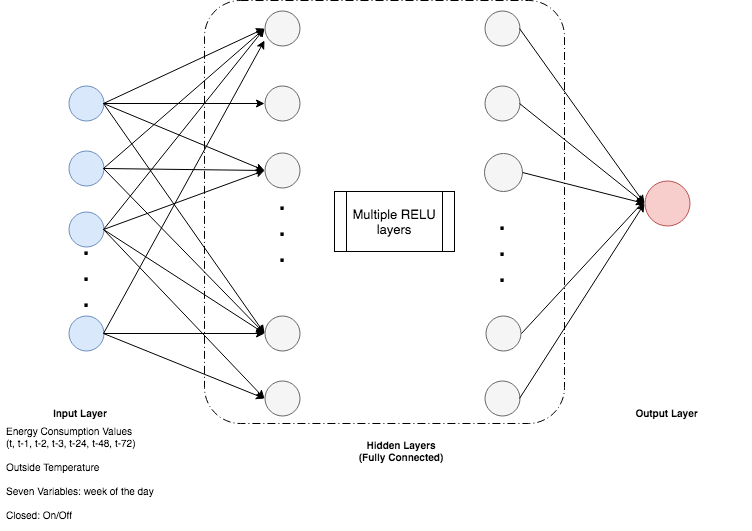
\includegraphics[width=4.5in, height=2.5in]{NN.png} 
  \caption{Neural Network Architecture} 
  \label{fig:example} 
\end{figure}

\section{Experimental Setup} \label{experiment}

\subsection{Cohort Selection} 
\indent The Historical Energy Consumption Data includes energy-use readings for over 200 buildings between that are sampled in different intervals over four years. Since our prediction task is to forecast next hour total building level energy use, we chose to train and test our model on the building that had the largest amount of hourly use data (34,704 hourly readings at SiteId 2). To train and test our model, we will use hourly energy readings of the same building. 

\subsection{Data Extraction}
\indent Our data set was given in four tables: Historical Consumption, Building Metadata, Holiday Information, and Weather Information. The features of each of these data tables is described below. 

\begin{table}[htbp]
\centering 
\begin{tabular}{ |c|c|c|c|} 
 \hline
 Historical Consumption & Building Metadata & Weather Information & Holiday Information \\ 
 \hline
 ObsId & SiteId & SiteId & Date \\  
 SiteId & Surface & Timestamp & Holiday \\ 
 Timestamp & Sampling & Temperature & SiteId \\ 
 ForcastId & Basetemperature & Distance & Index \\ 
 Value & On/Off for day of week &  &  \\
 \hline
\end{tabular}
 \label{tab:example} 
    \caption{Features From Different Raw Datasets.} 
\end{table}

From the Historical Consumption data, we created calculated columns that contain current energy consumption and energy consumption one hour ago, two hours ago, three hours ago, 24 hours ago, 48 hours ago and 72 hours ago. The inclusion of this historical data allows our neural network to have time series properties. 

Before, making our Timestamp data 24 hour periodic, we applied the lubridate package to extract the day of the week when each energy-use readings was recorded. In order to make the data 24 hour periodic, we pre-processed the Historical Consumption data's Timestamp feature with a basis function. To reflect the season and date changes, we used the Weather Information data and took the mean outside temperature for all readings at the particular SiteId, and Timestamp. Then we merged the temperature reading with the Historical Consumption data. 

From the Building Metadata and the day of week feature from the Historical Consumption data, we created a calculated column that describes whether or not the building was closed for that energy reading. 

For the Holiday dataset, we simply dropped all the features, because SiteId 2 does not have any energy readings that occur on a holiday. However, as indicated by Hippert et. al.\footnote{Hippert, Neural Networks, 44.}, holiday data improves short-load forecasts and should be included in other building prediction models. 

 \begin{figure}[!htbp]
  \centering 
  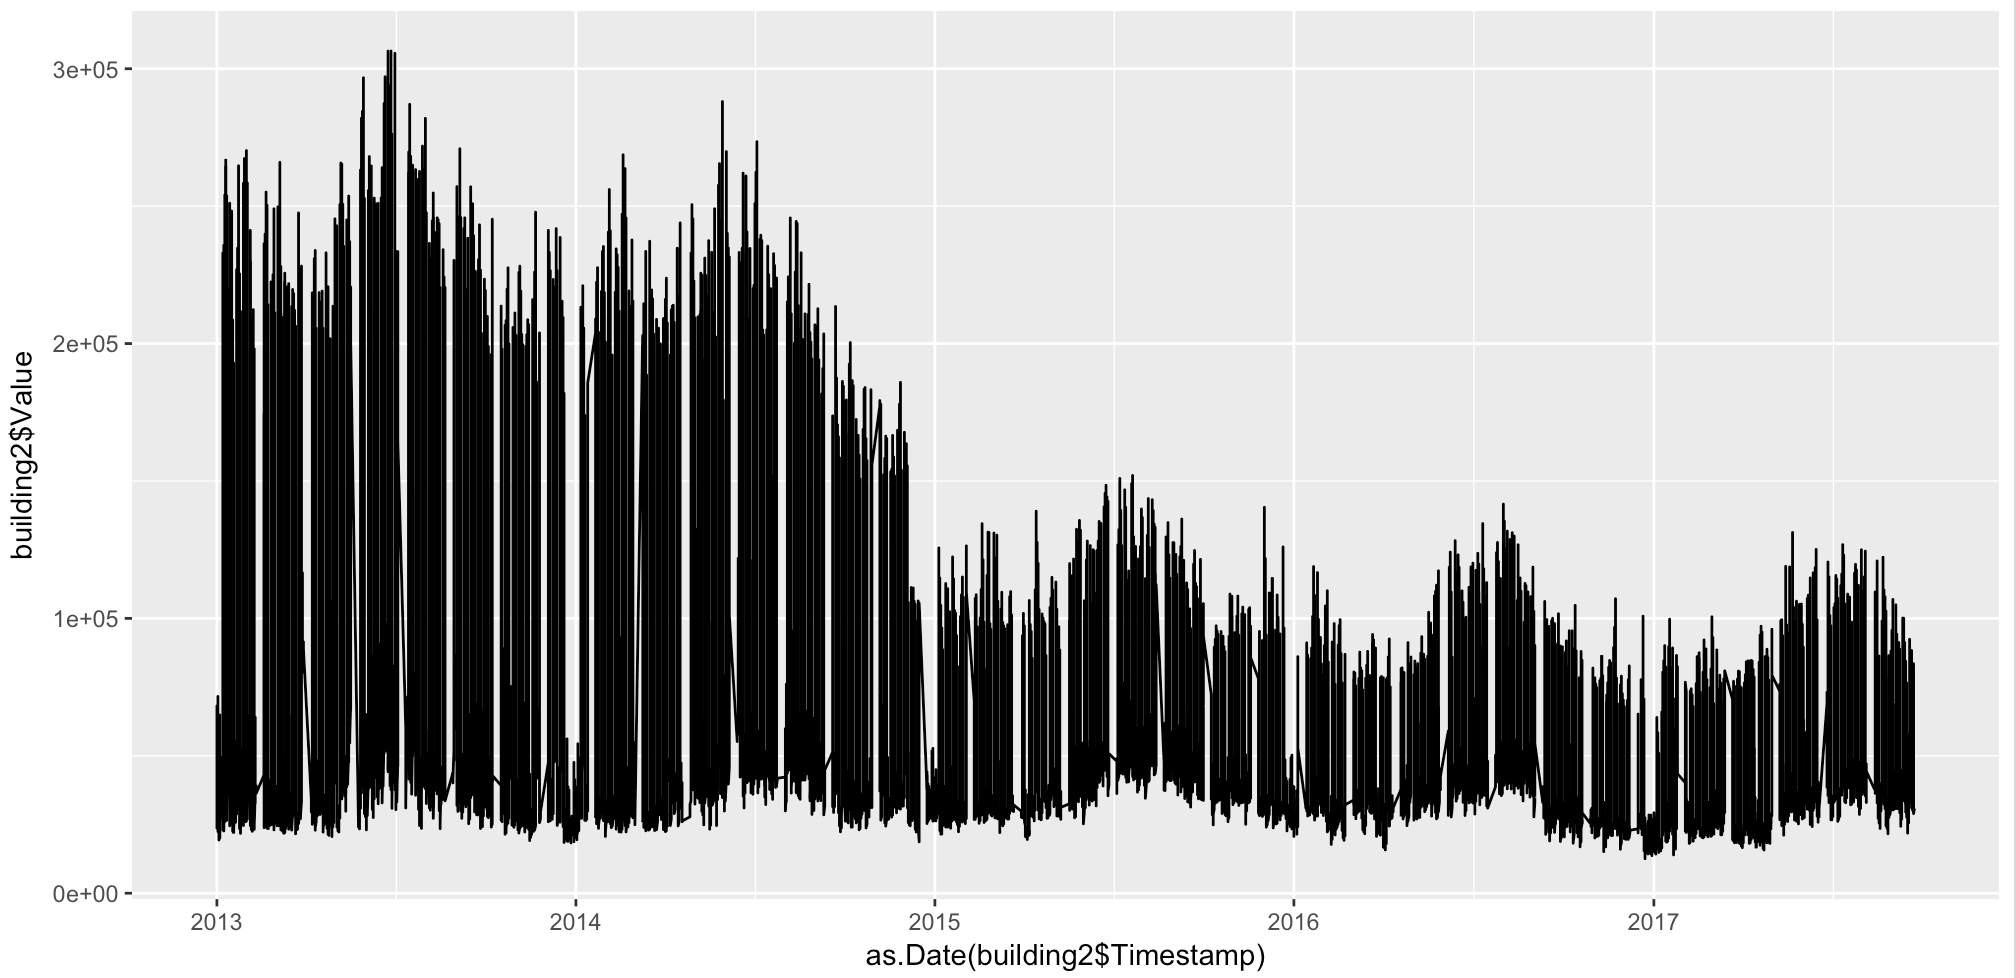
\includegraphics[width=4.5in, height=2.5in]{data_plot.png} 
  \caption{Energy Consumption Trend Over Five Years}
  \label{fig:example} 
\end{figure}
\FloatBarrier
Figure 4, demonstrates the hour energy use over a four year period. The chart illuminates the missing hourly energy readings, especially after year 2015. To address this problem, our first approach was to use the more complete years as training set and use the post-2015 data as the test set. However, after splitting the data, we found there's an unexplained drop in energy consumption after September 2015, and we could not use this method because our train set would be systematically different from our test set. To address this, we dropped all hourly energy-use readings that contained NA values.
\subsection{Feature Selection}

In addition to historical use, a building's energy consumption is closely related to the day of the week. To build this into our model, we added seven variables that capture the day of the week for each energy use reading. For example, we set Sunday to 1 and others as 0 to represent a day is Sunday. In addition, we extract data on whether the building is open or closed on that day from the Building Metadata table.

Furthermore, a building's outside temperature has tremendous impact on the building's hourly energy consumption value. This is due the relationship between temperature and the use of air conditioning and heating systems. To include outside temperature in our model, we extracted outside temperature data from the Weather Information Data. In the raw format, their are readings from multiple weather stations and we took the mean of each of these readings to provide one measure of outside temperature for each energy use reading. 

Lastly, to incorporate the historical hourly energy use readings into our model, we applied a basis function to convert our metering time-stamps into a cyclic format. We set the period for our basis transformation to 24 to represent each hour of the day.
\subsection{Feature Selection}
\begin{figure}[htbp]
  \centering 
  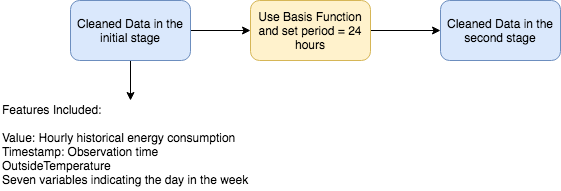
\includegraphics[width=4.5in]{1.png} 
  \caption{Adapt Basis Function}
  \label{fig:example} 
\end{figure}


Figure 6, summarizes the first data cleaning process which produced 11 variables for our feature matrix: \textit{Value} which represents the energy consumption within an hour, \textit{Hour} as represented by sin and cos features to indicate where the energy use reading is in the 24 hour cycle, \textit{OutsideTemperature} which represents average outside temperature at the energy use reading, and \textit{Sun, Mon, Tue, Wed, Thu, Fri} to indicate the day of the week.

\begin{figure}[!htbp]
  \centering 
  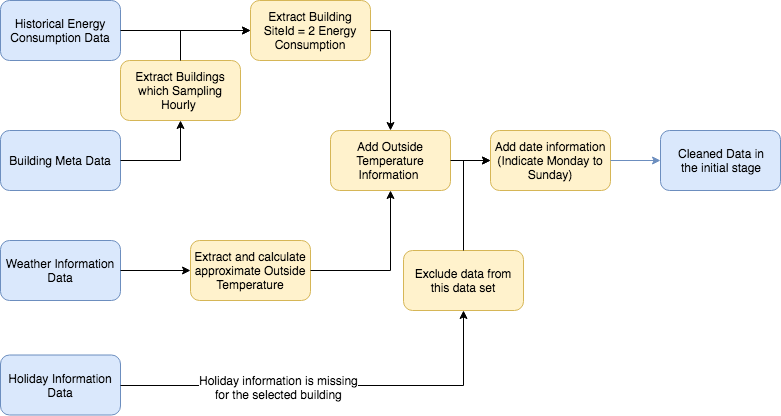
\includegraphics[width=4.5in, height=2.5in]{0.png} 
  \caption{Data Extraction Methods to Transform Raw Data for Model Development}
  \label{fig:example} 
\end{figure}
\FloatBarrier

As seen in Figure 7, to capture the relationship between historical energy use and our next hour energy use forecast, we went through a second round of data cleaning to incorporate lagged energy consumption effects into our prediction model. 

\begin{figure}[!htbp]
  \centering 
  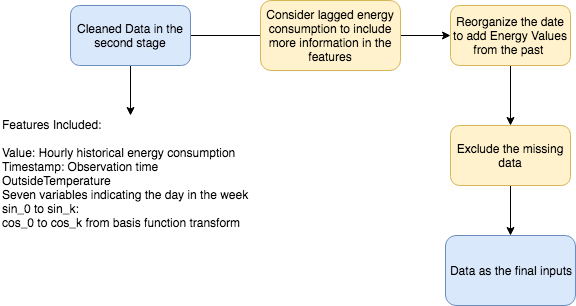
\includegraphics[width=4.5in]{2.png} 
  \caption{Consider Energy Consumption Lagged Effect}
  \label{fig:example} 
\end{figure}
\FloatBarrier

To determine these features, we made two assumptions (1) that the energy consumption values in the previous three hours' has a significant effect on next hour energy use, and (2) the next hour energy use will be similar to the energy use at that time in the past 24 hours', 48 hours' and 72 hours'. 

Therefore, we added these seven lagged use features and reorganized the data frame to obtain the final inputs to the neural network model. The input schema is as follows:

\begin{table}[!htbp]
\centering 
\begin{tabular}{ |c|c|c|c|c|c|}
\hline
\multicolumn{6}{|c|}{Final Input Feature} \\
 \hline
T72 & T48 & T24 & T3 & T2 & \\ 
 T1 & T0 & Sun & Mon & Tue & Wed\\ 
 Thu & Fri & Sat & Closed & OutsideTemperature & sin1\\ 
 sin2 & sin3 & sin4 & sin5 & cos1 & cos2\\ 
 cos3 & cos4 & cos5 &  &  & \\ 
 \hline
\end{tabular}
\label{tab:example} 
    \caption{All Final Input Features} 
\end{table}
\FloatBarrier

\subsection{Comparison Methods}

After training and testing the neural network model, we applied all of the same features to a linear regression. We did this to replicate the gains of using neural networks from the linear modeling used in the late 80's and early 90's. As suggested by our literature review, we found the mse of the linear regression prediction to be very high (mse = 2551249500). 

To try to produce a more reasonable mse, we ran a linear regression model using a regularization method. However, regularization only performs well in situations where bias is low and variance is high. As there's a huge bias in our training set, we were not to confident in our ability to reduce the mse. After running the model, our hypothesis held true and the mse after L1 regularization was 2547857458. So, we confirmed the understanding that short-term energy load forecasts are non-linear, and the energy consumption should not be predicted by a linear model.

\subsection{Evaluation Criteria}

The model's results are evaluated using cumulative value of coefficient of variant of root mean squared error(CV-RSME)[L1]. The equation is presented below:
\begin{figure}[htbp]
  \centering 
  \includegraphics[width=2.5in, height=1in]{rsme_equation.png} 
  \caption{CV-RSME Equation}
  \label{fig:example} 
\end{figure}

\section{Results} \label{results}

We conducted our neural network model using different training data sizes, such as 1/2, 1/3, 1/4...1/10 of the whole training data set. Our experiment found that the best prediction is produced by using the full training data set. We can find the final ANN prediction result in the figure below. We also can see the contrast result using different training data size in the figure below.

In addition, our network is compared to the linear regression model and as mentioned above, we evaluated the predictions by CV-RSME. The result can be found in the table below.

\begin{table}[!htbp]
  \centering 
  \begin{tabular}{lclc} 
    Method & CV-RSME (\%) \\ 
    \hline \\[-11pt]
    ANN & 7.5 \\ 
    Linear Regression & 50 \\ \hline 
  \end{tabular}
  \label{tab:example} 
\end{table}

\begin{figure}[!htbp]
  \centering 
  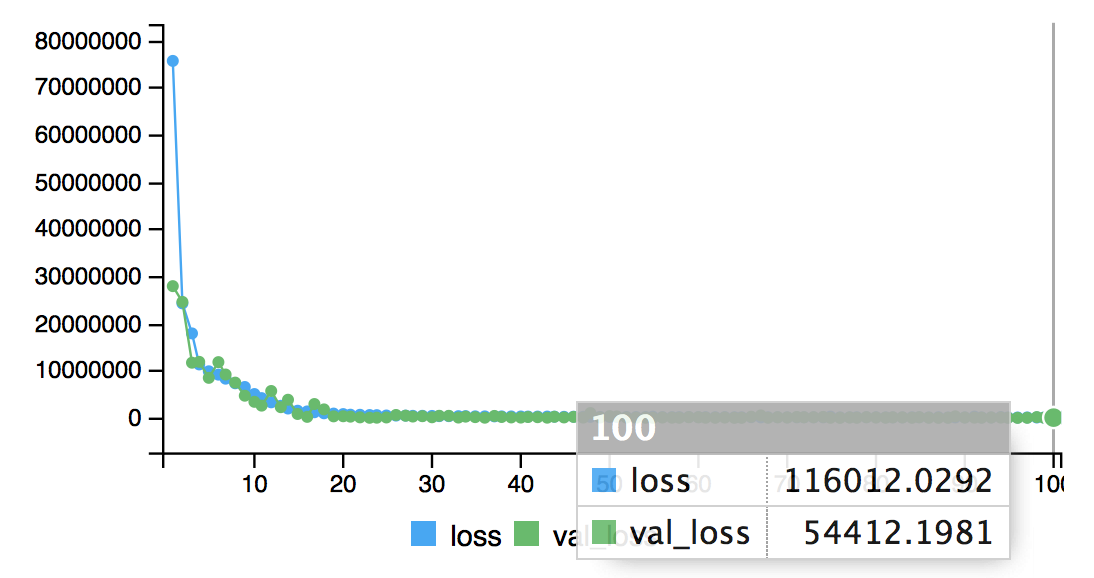
\includegraphics[width=4.5in, height=2.5in]{final_results.png} 
  \caption{Final Result Of ANN Prediction}
  \label{fig:example} 
\end{figure} 

\begin{figure}[!htbp]
  \centering 
  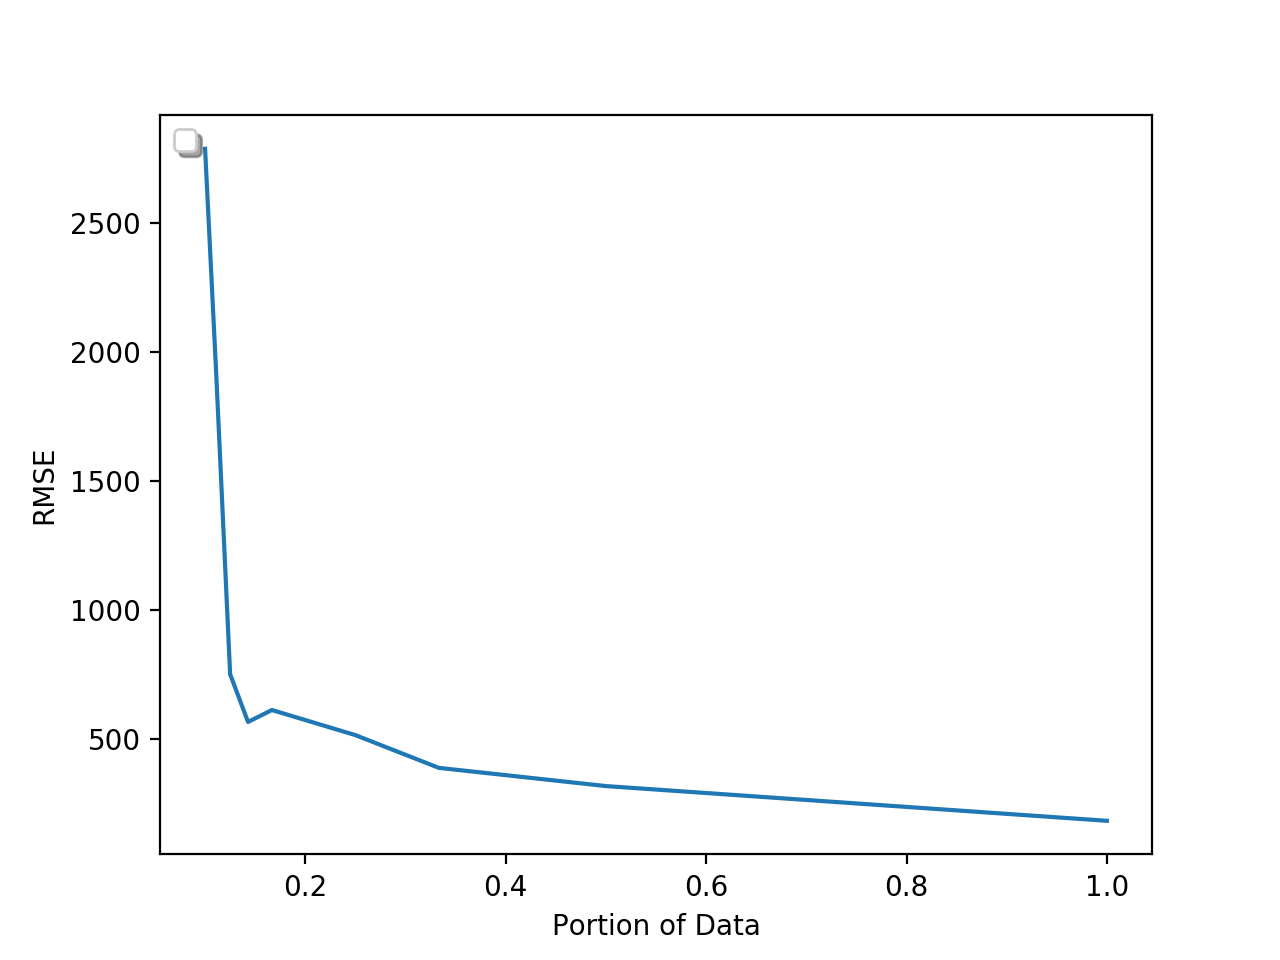
\includegraphics[width=4.5in, height=2.5in]{rmse_data.png} 
  \caption{RSME Results Of Different Training Size}
  \label{fig:example} 
\end{figure} 
\FloatBarrier

\section{Discussion and Related Work} 

Our results further proved that predicting short-term energy load requires a nonlinear prediction model. This can be seen by the reduction from 50\% CV-RSME with linear regression to 7.5\% CV-RSME with our ANN model. Our model contributes to the field because it focuses on a single building forecast which will be in higher demand as distributed energy systems and microgrids increase in popularity\footnote{Amjady et. al. Forecast of Microgrids, 286.}. 

Despite the low CV-RSME for a volatile output vector, our model can be improved. First, for the model to be learned by other building data, it needs to account for Holiday data because it has been shown to affect energy consumption. Second, to prepare our data for analysis we removed energy-use readings that contained NA values before we calculated our T-x features. This means that T-3 may not represent energy-use three hours ago for all observations. Instead, it could refer to T-4 if one observation between T-1 and T-4 contained an NA value. Additionally, our model may have ommitted some other important features that have a big effect on energy consumption. Lastly, our model is focused on hourly energy-use readings of electricity for one building and may not apply to other utility usage such as natural gas and water or electricity usage of a different building. 

Overall, with improved building short-term load forecasts, push back from utility companies and consumer advocates on microgrid technology will decrease. This is because the revenue model for utilities is driven by matching supply with demand.\footnote{Hippert, Neural Networks, 44.} So, improving forecasts increases their confidence in being able to supply energy without the backing of a national energy transmission system. Additionally, consumer advocates will become more supportive of microgrid technology because the threat of unstable energy access under distributed systems will be reduced. 

\section{Conclusion} 
Utility companies have been interested in predicting short-term energy load for the past 30 years. This interest has been driven by changes in the energy industry. Today, energy transmission is transitioning into a microgrid structure. This shift will continue to substantiate the need for more accurate short-term energy load predictions at the building level. Our research compared partition based machine learning algorithms and neural networks to further demonstrate the superiority of non-linear forecasting in energy prediction. In addition, our ANN model's ability to account for and iteratively learn weights for historical data is innovative and should serve as a baseline for volatile energy use predictions models. To extend this model, statisticians and computer scientists should apply it to other buildings. A targeted approach for this extension would be to model next hour energy-use for all buildings in a location testing microgrid technologies. This research setting would ensure the models applicability to the incoming electricity transmission infrastructure. 

% ACKNOWLEDGEMENTS
% \acks{Many thanks to all collaborators and funders!}

\bibliography{sample}
\indent Figure 1. Image Source: https://www.pyimagesearch.com/wp-content/uploads/2016/08/simple_neural_network_header.jpg

Figure 2. Image Source: Applied Analytics: the Machine Learning Pipeline neural network notes
\appendix


\end{document}
